% !Rnw weave = knitr
\documentclass[a4paper, french, 11 pt]{article}\usepackage[]{graphicx}\usepackage[]{xcolor}
% maxwidth is the original width if it is less than linewidth
% otherwise use linewidth (to make sure the graphics do not exceed the margin)
\makeatletter
\def\maxwidth{ %
  \ifdim\Gin@nat@width>\linewidth
    \linewidth
  \else
    \Gin@nat@width
  \fi
}
\makeatother

\definecolor{fgcolor}{rgb}{0.345, 0.345, 0.345}
\newcommand{\hlnum}[1]{\textcolor[rgb]{0.686,0.059,0.569}{#1}}%
\newcommand{\hlstr}[1]{\textcolor[rgb]{0.192,0.494,0.8}{#1}}%
\newcommand{\hlcom}[1]{\textcolor[rgb]{0.678,0.584,0.686}{\textit{#1}}}%
\newcommand{\hlopt}[1]{\textcolor[rgb]{0,0,0}{#1}}%
\newcommand{\hlstd}[1]{\textcolor[rgb]{0.345,0.345,0.345}{#1}}%
\newcommand{\hlkwa}[1]{\textcolor[rgb]{0.161,0.373,0.58}{\textbf{#1}}}%
\newcommand{\hlkwb}[1]{\textcolor[rgb]{0.69,0.353,0.396}{#1}}%
\newcommand{\hlkwc}[1]{\textcolor[rgb]{0.333,0.667,0.333}{#1}}%
\newcommand{\hlkwd}[1]{\textcolor[rgb]{0.737,0.353,0.396}{\textbf{#1}}}%
\let\hlipl\hlkwb

\usepackage{framed}
\makeatletter
\newenvironment{kframe}{%
 \def\at@end@of@kframe{}%
 \ifinner\ifhmode%
  \def\at@end@of@kframe{\end{minipage}}%
  \begin{minipage}{\columnwidth}%
 \fi\fi%
 \def\FrameCommand##1{\hskip\@totalleftmargin \hskip-\fboxsep
 \colorbox{shadecolor}{##1}\hskip-\fboxsep
     % There is no \\@totalrightmargin, so:
     \hskip-\linewidth \hskip-\@totalleftmargin \hskip\columnwidth}%
 \MakeFramed {\advance\hsize-\width
   \@totalleftmargin\z@ \linewidth\hsize
   \@setminipage}}%
 {\par\unskip\endMakeFramed%
 \at@end@of@kframe}
\makeatother

\definecolor{shadecolor}{rgb}{.97, .97, .97}
\definecolor{messagecolor}{rgb}{0, 0, 0}
\definecolor{warningcolor}{rgb}{1, 0, 1}
\definecolor{errorcolor}{rgb}{1, 0, 0}
\newenvironment{knitrout}{}{} % an empty environment to be redefined in TeX

\usepackage{alltt}
\usepackage[T1]{fontenc}
\usepackage[utf8]{inputenc}
\usepackage{lmodern}
\usepackage{textcomp}
\usepackage[french]{babel}
\usepackage{geometry}
\geometry{top=1cm, bottom=1cm, left=1cm, right=1cm}
\usepackage{graphicx}
\usepackage{epstopdf}
\usepackage{booktabs}
\usepackage[skip=0.5\baselineskip]{caption}

\epstopdfDeclareGraphicsRule{.gif}{png}{.png}{convert gif:#1 png:\OutputFile}
\AppendGraphicsExtensions{.gif}

\title{Titre provisoire}
\author{Louis Bourges, Jean-Baptiste Lagrange-Dupuis et Luc Letonturier}
\date{\today}
\IfFileExists{upquote.sty}{\usepackage{upquote}}{}
\begin{document}

\maketitle

Et ici on peut écrire ... et insérer des blocs de code qui s'éxécutent, avec le code et le résultat qui s'affichent

\begin{knitrout}
\definecolor{shadecolor}{rgb}{0.969, 0.969, 0.969}\color{fgcolor}\begin{kframe}
\begin{alltt}
\hlstd{a} \hlkwb{<-}  \hlnum{2}\hlopt{+}\hlnum{2}
\hlstd{a}
\end{alltt}
\begin{verbatim}
## [1] 4
\end{verbatim}
\end{kframe}
\end{knitrout}

ou juste le résultat : 

\begin{knitrout}
\definecolor{shadecolor}{rgb}{0.969, 0.969, 0.969}\color{fgcolor}\begin{kframe}
\begin{verbatim}
## [1] 6
\end{verbatim}
\end{kframe}
\end{knitrout}

ou totalement invisibles : 


Et ensuite on peut citer les résultats : à première vue $4 < 6$ mais je crois que c'est 8 qui est le plus grand.


Un petit graphique : 



\begin{figure}[h]
\center
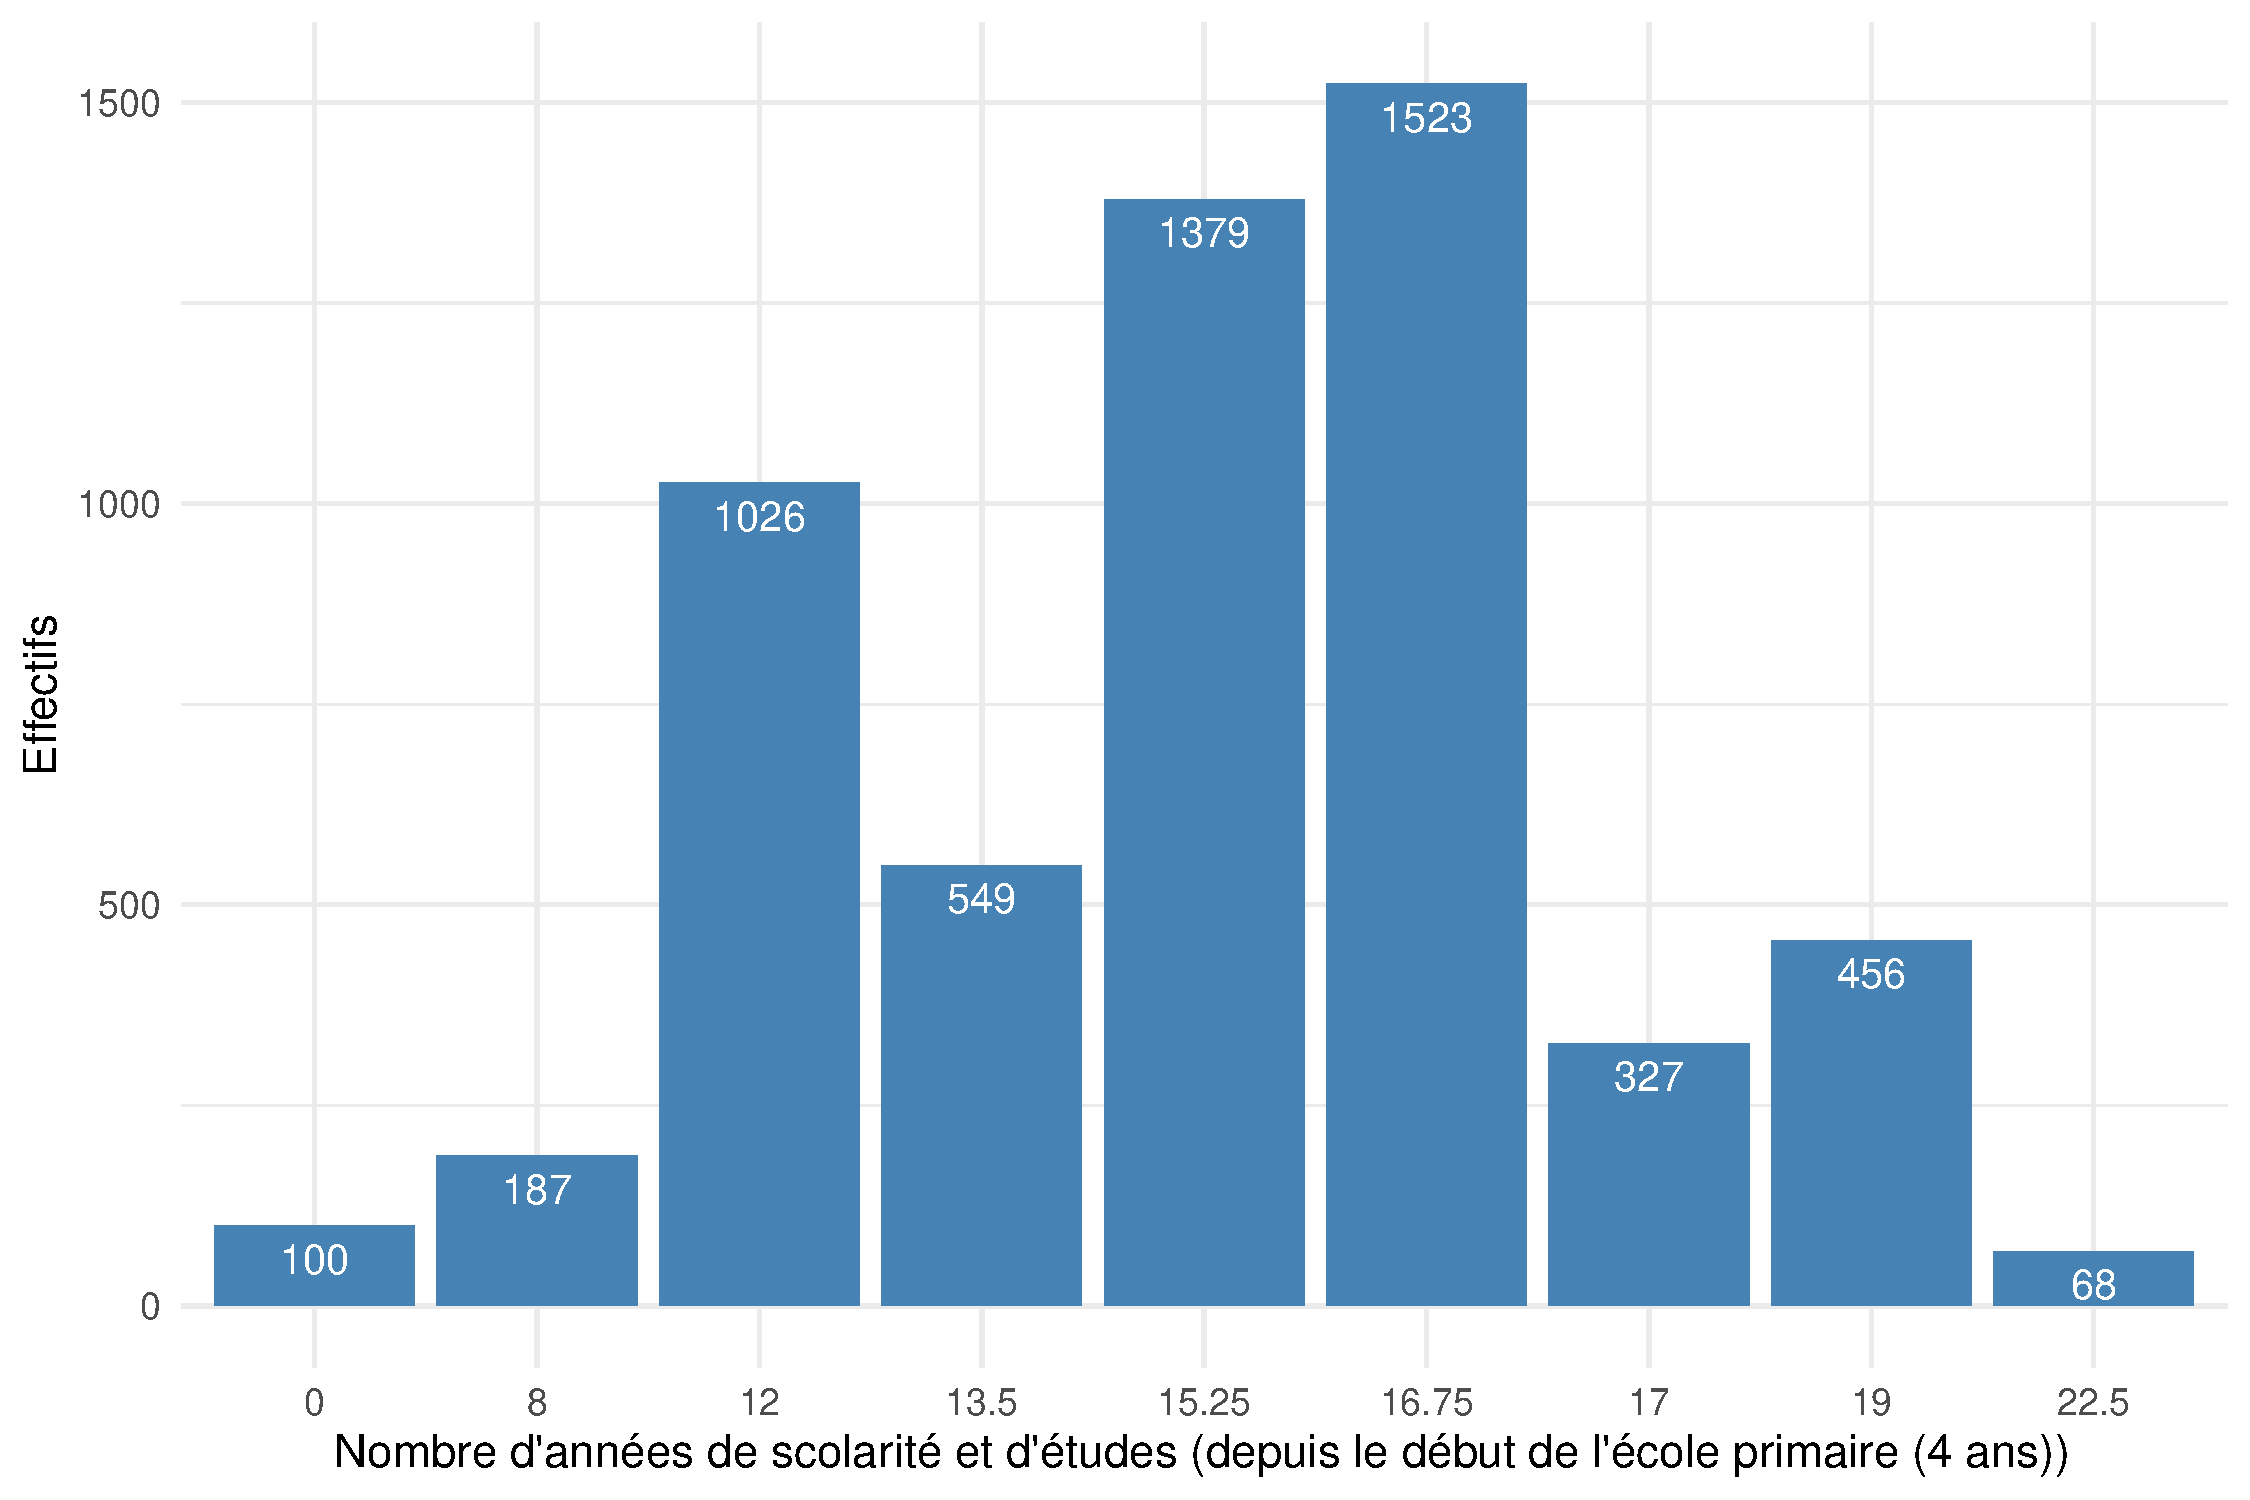
\includegraphics[width=0.7\linewidth]{figure/educ.pdf}
\caption{Niveau d'éducation (avec diplôme) des individus de l'échantillon}
\end{figure}

\begin{knitrout}
\definecolor{shadecolor}{rgb}{0.969, 0.969, 0.969}\color{fgcolor}\begin{kframe}
\begin{verbatim}
## [1] 5615
## [1] 0
\end{verbatim}
\end{kframe}
\end{knitrout}


% latex table generated in R 4.2.1 by xtable 1.8-4 package
% Sun May 14 03:04:22 2023
\begin{table}[ht]
\centering
\caption{Tableau des résidus} 
\label{tb:lm1}
\begin{tabular}{rrrrr}
  \toprule
 & Estimate & Std. Error & t value & Pr($>$$|$t$|$) \\ 
  \midrule
(Intercept) & 5.6786 & 0.1095 & 51.84 & 0.0000 \\ 
  data\$age & 0.0072 & 0.0010 & 7.11 & 0.0000 \\ 
  data\$genre & -0.3039 & 0.0225 & -13.53 & 0.0000 \\ 
  data\$heures & 0.0142 & 0.0008 & 17.03 & 0.0000 \\ 
  data\$experience & 0.0024 & 0.0011 & 2.15 & 0.0316 \\ 
  data\$nbenfants & -0.0097 & 0.0096 & -1.01 & 0.3112 \\ 
  data\$education & 0.1083 & 0.0059 & 18.44 & 0.0000 \\ 
   \bottomrule
\end{tabular}
\end{table}



\end{document}
